% This is a LaTeX input file.
%
% A '%' character causes TeX to ignore all remaining text on the line,
% and is used for comments like this one.

\documentclass[a4paper]{article}      % Specifies the document class

                             % The preamble begins here.
\title{Rank parameters for Bland--Altman plots}  % Declares the document's title.
\author{Roger B. Newson}      % Declares the author's name.
%\date{21~May, 2018}      % Deleting this command produces today's date.

\newcommand{\ip}[2]{(#1, #2)}
                             % Defines \ip{arg1}{arg2} to mean
                             % (arg1, arg2).

%\newcommand{\ip}[2]{\langle #1 | #2\rangle}
                             % This is an alternative definition of
                             % \ip that is commented out.

\usepackage{graphics}
\usepackage{hyperref}

%
% Set margins
% (which are explained in Figure C3 of LaTeX User's Guide
% and which CAN BE RESET BY EDITORS AT ANY TIME AS FAR AS I CARE!!!!!!!!
% - RBN.)
%
\setlength{\topmargin}{-0.5in}
%\setlength{\headsep}{0.25in}
\setlength{\oddsidemargin}{0in}
\setlength{\evensidemargin}{0in}
\setlength{\textwidth}{6.5in}
\setlength{\textheight}{10in}

%
% Set page style (headers and footers)
%
\pagestyle{myheadings}
\markboth{\textit{Rank parameters for Bland--Altman plots}}
{\textit{Rank parameters for Bland--Altman plots}}

\begin{document}             % End of preamble and beginning of text.

\maketitle                   % Produces the title.

\section{Introduction}

Bland--Altman plots were introduced by Altman and Bland (1983)\cite{altmanbland1983}
and popularized by Bland and Altman (1986)\cite{blandaltman1986}.
Given $N$ bivariate data points $(A_i,B_i)$,
expressed in the same units
and assumed to be two alternative quantities used to measure the same thing (such as exam marks of the same students allocated by Lecturers~$A$ and $B$),
a Bland--Altman plot is derived by rotating the scatter plot of the $A_i$ (on the vertical axis) and the $B_i$ (on the horizontal axis)
through 45 degrees by transforming the bivariate column vectors $(A_i,B_i)^T$ with the rotation matrix
\begin{equation}
R = \left[
\begin{array}{rr}
1&-1 \\
{1\over 2}&{1\over 2}
\end{array}
\right].
\label{eq:eqseq1}
\end{equation}
Alternatively, in simpler language,
it is defined by plotting the differences $A_i-B_i$ on the vertical axis
against the means $(A_i + B_i)/2$ on the horizontal axis.

The Bland--Altman plot is a good graphical summary of the paired data points $(A_i,B_i)$.
However, we might prefer also to have confidence intervals for parameters of the Bland--Altman plot,
in order to be able to make quantitative statements on how the $A_i$ and the corresponding $B_i$
agree and/or disagree with each other.
In Section~4.7 of van Belle (2008)\cite{vanbelle2008},
it is argued (following Lin (1989)\cite{lin1989})
that the three principal components of disagreement are discordance (also known as "imprecision"), bias, and scale differential.
Suppose that the $(A_i,B_i)$ are sampled from a common bivariate distribution,
with means $\mu_a$ and $\mu_B$, standard deviations $\sigma_A$ and $\sigma_B$,
and correlation coefficient $\rho_{AB}$.
Disagreement can then be decomposed into these three components by the formula
\begin{equation}
{{E[(A-B)^2]}\over{2\sigma_A\sigma_B}} \, = \, (1-\rho_{AB}) \, + \, {{(\mu_A-\mu_B)^2}\over{2\sigma_A\sigma_B}} \, + \, {{(\sigma_A-\sigma_B)^2}\over{2\sigma_A\sigma_B}} ,
\label{eq:eqseq2}
\end{equation}
where the left--hand side measures general disagreement,
the first term in the right--hand side measures discordance,
the second term in the right--hand side measures squared bias,
and the third term in the right-hand side measures squared scale differential.

It will be argued here that all three principal components of disagreement are better measured using rank parameters than using regression parameters,
although the regression parameters may be good proxies for the rank parameters if the $(A_i,B_i)$ are sampled
from a bivariate Normal distribution.
This is because the rank parameters are less influenced by outlying data points,
and also easier to interpret in words as measuring the appropriate type of disagreement.
The rank parameters used will be Kendall's~$\tau_a$, estimated using the methods of Newson (2006a)\cite{newson2006a},
and median differences, estimated using the methods of Newson (2006b)\cite{newson2006b}.

\subsection{Example dataset: Double marking of exam candidates}

We will demonstrate the methods using an example dataset with one observation for each of 179 candidates
in a medical school statistics examination,
and data on marks awarded by 2 academics,
who we will call ``Lecturer~$A$'' and ``Lecturer~$B$''.
Lecturer~$A$ was the more experienced of the two,
and Lecturer~$B$ was marking exams for the first time
(in the course of an all-night session on heavy doses of coffee).
There were 5 questions posed in the exam,
of which students were asked to attempt 4.
Each academic awarded each student a total mark,
equal to the sum of the student's marks on the best 4 questions attempted.
(It was not unknown for a student to attempt all 5 questions.)
3 of the candidates did not sit the exam,
leaving 176 students who could be marked.
Students were finally awarded the mean of the marks awarded by the two academics.
The results are analysed using the Stata statistical software\cite{statacorp},
particularly the add--on package \texttt{somersd}\cite{newson2006a}\cite{newson2006b},
and two other add--on packages \texttt{scsomersd} and \texttt{rcentile} (Newson, 2014)\cite{newson2014},
which depend on \texttt{somersd}.

\begin{figure}[htbp]
\caption{Scatter plot of marks awarded by Lecturers~$A$ and $B$.}
\label{figure:figseq1}
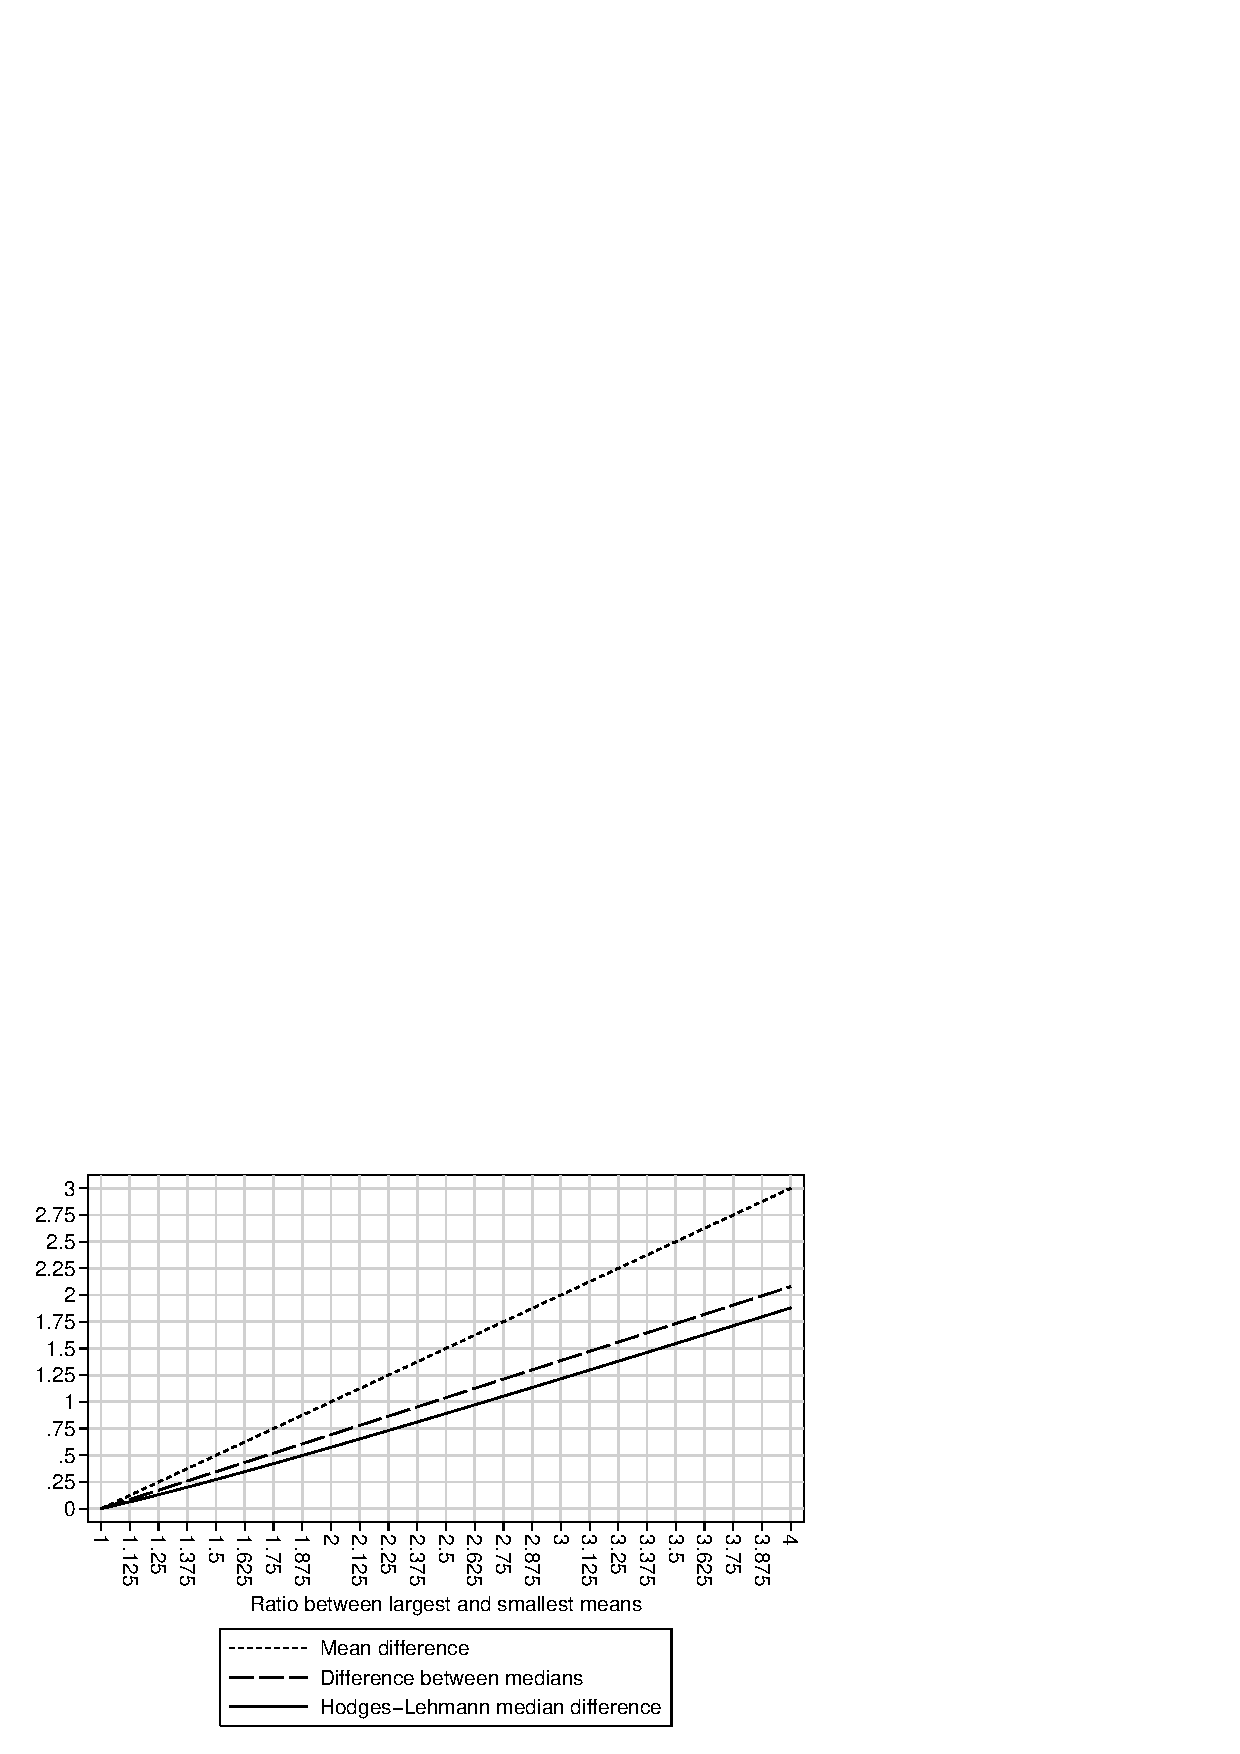
\includegraphics{figseq1.pdf}
\end{figure}

\begin{figure}[htbp]
\caption{Bland--Altman plot of marks awarded by Lecturers~$A$ and $B$.}
\label{figure:figseq2}
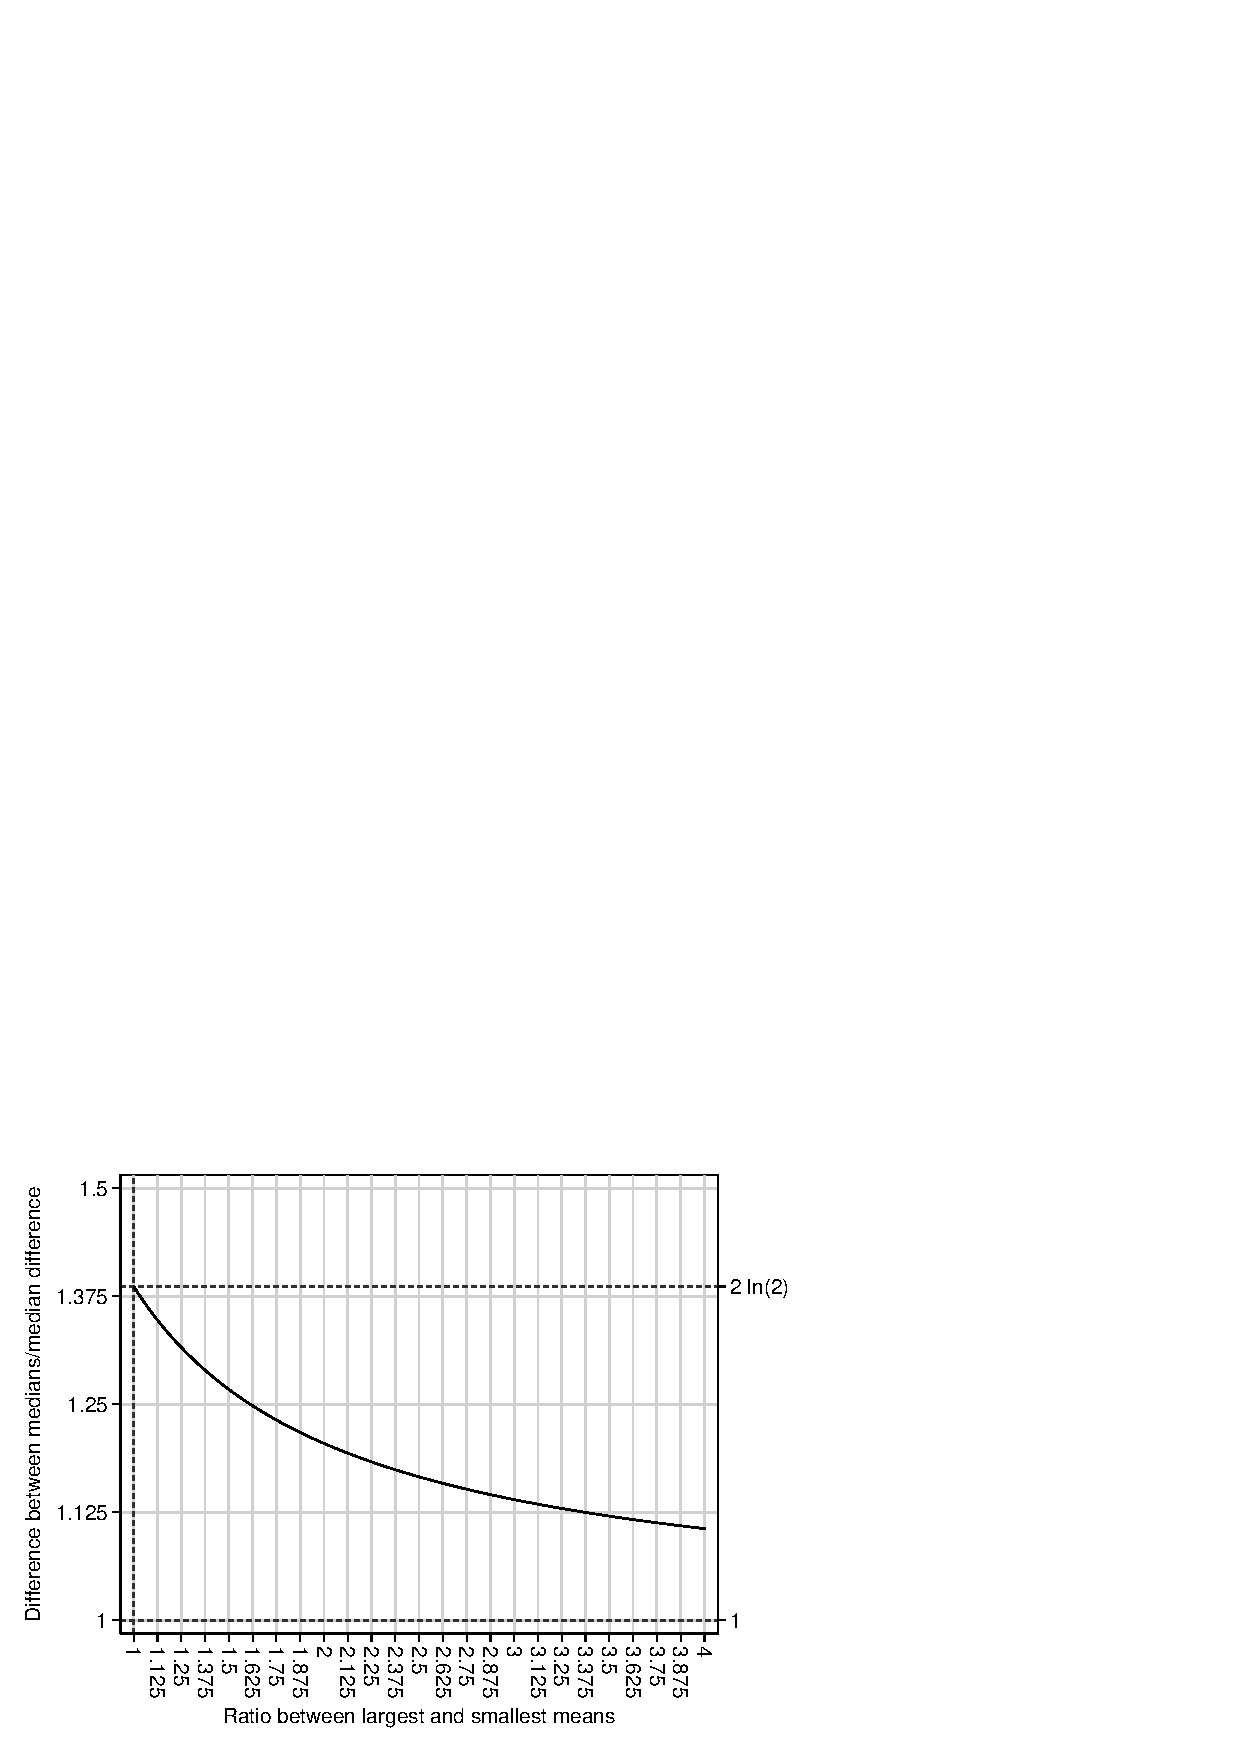
\includegraphics{figseq2.pdf}
\end{figure}

Figure~\ref{figure:figseq1} gives a scatter plot of the mark awarded by Lecturer~$A$
against the mark awarded by Lecturer~$B$.
Figure~\ref{figure:figseq2} gives a Bland--Altman plot
of the difference between the mark awarded by Lecturer~$A$
and the mark awarded by Lecturer~$B$
against the mean of the two marks (eventually awarded to the student).
The vertical--axis reference line at zero in Figure~\ref{figure:figseq2}
corresponds to the diagonal line of equality in Figure~\ref{figure:figseq1}.
Note that the Bland--Altman plot is more efficient in using space,
as there is no wasted space in the top left and bottom right parts of the plot region.
This allows us to view the vertical axis of the Bland--Altman plot in greater detail.
In particular, we can see that the differences are integer, instead of being continuous.

\section{Discordance parameters}

We assume a population of indexed individuals, with 2 scalar variables $X$ and $Y$ defined for each individual,
and a sampling scheme for sampling pairs of individuals (indexed as $i$ and $j$) at random from that population.
Kendall's $\tau_a$ of $X$ and $Y$ is then defined as
\def\sign{{\rm sign}}
\begin{equation}
\tau(X,Y) = E\left[ \sign(X_i-X_j) \sign(Y_i-Y_j) \right],
\label{eq:eqseq3}
\end{equation}
where $E(\cdot)$ denotes expectation,
and $\sign(x)$ is 1 if $x>0$, -1 if $x<0$, and 0 if $x=0$.
Alternatively, if we define the ``cordance sign''
\def\csign{{\rm csign}}
\begin{equation}
\csign(x_i,y_i,x_j,y_j) = \sign(x_i-x_j) \sign(y_i-y_j),
\label{eq:eqseq4}
\end{equation}
then we can define
\def\Pr{{\rm Pr}}
\begin{equation}
\tau(X,Y) = \Pr\left[ \csign(X_i,Y_i,X_j,Y_j)=1] - \Pr[\csign(X_i,Y_i,X_j,Y_j)=-1 \right],
\label{eq:eqseq5}
\end{equation}
where $\Pr(\cdot)$ is the probability of an event. In other words, $\tau(X,Y)$ is the difference between the probabilities of
\textbf{concordance} $(\csign(X_i,Y_i,X_j,Y_j)=1)$ and \textbf{discordance} $(\csign(X_i,Y_i,X_j,Y_j)=-1)$.

Returning to our variables $(A_i,B_i)$,
which are \textix{usually} assumed to be sampled independently and identically from a common population of indexed individuals
with a common bivariate distribution,
we might view $\tau(A,B)$ as a measure of the concordance component of agreement
and/or of the discordance component of disagreement.
If the indexed population is a population of students,
and $(A_i,B_i)$ is the numbers of exam marks awarded by Lecturers~$A$ and $B$ respectively,
then $\tau(A,B)$ is the difference between the probability that they agree and the probability that they disagree,
assuming that they are given 2 different exam scripts at random and are both asked which one is the best.
Specifically, in the 176 students with total marks,
the Kendall's $\tau_a$ between the $A_i$ and the $B_i$ is 0.708 (95\% CI, 0.649 to 0.758; $P=2.6\times 10^{-36}$).
So, with the 176 students in our sample, the two lecturers were 70.8 percent more likely to agree than to disagree.
And, in the population of students at large, from which these 176 students were sampled,
we are 95\% confident that the two lecturers would be 64.9\% to 75.8\% more likely to agree than to disagree.
(This confidence interval is asymmetric because it was computed using the Normalizing hyperbolic arctangent or Fisher's~$z$ transformation.)
And the $P$--value shows that,
in a fantasy scenario in which the lecturers were equally likely to agree or to disagree
about pairs of students sampled randomly from the population at large,
such a level of agreement in a sample would be \textit{very} rare.

Returning to Figures~\ref{figure:figseq1} and \ref{figure:figseq2},
we note that the scatter plot of Figure~\ref{figure:figseq1} draws attention to concordance/discordance,
because it has empty space in the upper left and lower right parts of the plot region,
and therefore draws attention to the fact that students with a higher $A_i$ from Lecturer~$A$
\textit{usually} also have a higher $B_i$ from Lecturer~$B$.
As we shall see,
the Bland--Altman plot of Figure~\ref{figure:figseq2}
draws attention to the other two components of agreement/disagreement.

\subsection{Kendall's $\tau_a$ \textit{versus} Pearson correlation}

Statisticians are frequently heard to assert that the Pearson correlation coefficient ``does not measure agreement''.
\textit{However}, \textit{if} a bivariate $(X,Y)$ is sampled from a bivariate Normal distribution,
or from any other bivariate distribution that can be transformed to bivariate Normal
using a pair of monotonic transformations $g(X)$ and $h(Y)$ that may or may not be identity transformations,
\textit{then} the Pearson correlation coefficient between the variables
(transformed if necessary)
is equal to
\begin{equation}
\rho[g(X),h(Y)] = \sin\left[ {\pi\over 2} \tau(X,Y) \right].
\label{eq:eqseq6}
\end{equation}
(Note that we do not have to know the form of $g(\cdot)$ and $h(\cdot)$ in order for this to apply.
Note, also, that this relation is monotonically increasing, and invertible,
over the closed interval from -1 to 1.)
This relation is known as \textbf{Greiner's relation},
and is discussed in Kendall (1949)\cite{kendall1949},
where it is pointed out that it also applies to a wide range of non--Normal bivariate distributions.
Therefore, under a wide range of assumptions,
the Pearson product--moment correlation $\rho(A,B)$ may measure at least one component of agreement/disagreement
between the $A_i$ and the $B_i$,
namely concordance/discordance.
\textit{However}, it does this in an indirect way,
which cannot be interpreted simply as a difference between probabilities of agreement and disagreement.

In our example dataset, the Pearson correlation between the marks awarded by the two lecturers,
estimated using Greiner's relation to transform the estimate and confidence limits for Kendall's~$\tau_a$,
was 0.896 (95\% CI, 0.852 to 0.928).
This is in good agreement with the directly--estimated Pearson correlation of 0.908.
Under Greiner's relation, the Pearson correlation has a higher magnitude than the corresponding Kendall's~$\tau_a$.
It is therefore important for the audience to understand the meaning of Kendall's~$\tau_a$
as a difference between concordance and discordance probabilities.
They should not become confused,
just because they are accustomed to the higher--magnitude Pearson correlations and
find the lower--magnitude Kendall's~$\tau_a$ less impressive.

\section{Bias parameters}

The second component of disagreement is bias,
which we commonly measure using a paired $t$--test
to derive a confidence interval for the mean of the differences $A_i-B_i$.
A possible alternative measure of bias might be percentile differences
between the $A_i$ and $B_i$.
We can estimate the median (equal to the mean in a bivariate Normal model),
and also other percentiles,
to show how differences between measurements on the same subject
vary within the population of subjects.

A useful Stata package for measuring percentiles is \texttt{rcentile} (Newson, 2014)\cite{newson2014},
which allows adjustment of confidence intervals for clustering and/or weighting if necessary,
and also saves the confidence intervals conveniently in a Stata matrix for the user to use.
(In default, these confidence intervals for percentiles are calculated using the Normalizing and variance--stabilizing
hyperbolic arctangent or Fisher's~$z$ transform
on the mean signs of the differences between data values and percentiles.)

\begin{figure}[htbp]
\caption{Percentile differences between marks awarded to the same candidate by Lecturers~$A$ and $B$.}
\label{figure:figseq3}
\includegraphics{figseq3.pdf}
\end{figure}

\begin{table}[htbp]
\caption{Percentile differences between marks awarded to the same candidate by Lecturers~$A$ and $B$.}
\begin{tabular}{rrrr}
\textit{Percent}&\textit{Percentile}&\textit{(95\%}&\textit{CI)}\\
0&-8&(-8,&-8)\\
12.5&-1&(-2,&-1)\\
25&0&(-1,&1)\\
37.5&1&(1,&2)\\
50&2&(2,&3)\\
62.5&3&(3,&4)\\
75&4&(4,&4)\\
87.5&5&(5,&6)\\
100&8&(8,&8)\\
\end{tabular}
\label{table:tabseq1}
\end{table}

In our example dataset, the percentile differences in marks awarded to the same candidate by Lecturers~$A$ and $B$
are plotted against percents (with increments of 12.5\% or 1/8)
in Figure~\ref{figure:figseq3}.
They are also tabulated in Table~\ref{table:tabseq1}.
Note that, for most of the percentiles,
the upper and/or lower 95\% confidence limits are equal to the estimate.
This is a consequence of the fact that the differences are all integers,
implying that percentile differences and their confidence limits can only be integers or half-integers.
However, this does not invalidate the confidence intervals,
except in the case of Percentiles~0 and 100,
which are the minimum and maximum, respectively,
and which are not covered by the Central Limit Theorem.
We see that, most of the time, Lecturer~$A$ is ``Mr Nice'',
who allocates a higher mark than Lecturer~$B$ to the same student.
\textit{However}, Percentiles~12.5 and 25 indicate that, \textit{sometimes}, Lecturer~$B$ is more generous.
The paired $t$--test  on these data gave a mean difference
of 2.04 (95\% CI, 1.62 to 2.46; $P=9.3 \times 10^{-18}$).
This  tells us the positive \textit{mean} difference,
but does not tell us about the minority of exceptional negative differences.

\subsection{Tests and confidence limits for the mean sign}

Confidence intervals for percentiles do not always come with $P$--values.
\textit{However}, in this case, the parameter to test for a zero value is the mean sign,
defined as $E[\sign(A_i-B_i)]$.
This is the parameter tested by the sign test.
It can be  estimated, with confidence limits and a $P$--value,
using the \texttt{scsomersd} package in Stata,
which can be downloaded from the Statistical Software Components (SSC) archive,
and which requires two other SSC packages (\texttt{somersd} and \texttt{expgen}) in order to work.

To estimate the mean sign of the difference,
assuming that the difference itself is stored in a variable named \texttt{dtotmark},
we type, in Stata,
\begin{equation}
\mbox{\texttt{scsomersd dtotmark 0, transf(z) tdist}}
\label{eq:eqseq8}
\end{equation}
and the mean sign is displayed with confidence limits and a $P$--value,
once again using the hyperbolic arctangent or Fisher's~$z$ transformation.
In our data,
it is 0.534 (95\% CI, 0.404 to 0.643; $P=5.1\times 10^{-11}$).
This means that, in our sample,
Lecturer~$A$ awarded the higher mark 53.4\% more often than Lecturer~$B$ awarded the higher mark.
And, in the population from which these students were sampled,
the former event would happen 40.4\% to 64.3\% more often than the latter event.
And the $P$--value shows that a mean sign of this magnitude would very rarely happen by chance,
if both lecturers were equally likely to award the higher mark.

Looking at the Bland--Altman plot of Figure~\ref{figure:figseq2}),
we get the impression that there are more data points above the line of zero difference than below the line of zero difference.
The mean sign, and the percentile differences, support this impression.

\section{Scale differential parameters}

Two methods may also disagree on the scale of the differences between values.
In our example dataset, we might ask whether Lecturer~$A$ or Lecturer~$B$ awarded marks
that differed more,
generating a greater difference between the better exam scripts and the worse exam scripts.

A good estimate of this tendency, using rank methods, is
\begin{equation}
\tau[A-B,(A+B)/2] \, = \, \tau(A-B,A+B) \, ,
\label{eq:eqseq9}
\end{equation}
which is the difference between the probabilities of concordance and discordance between
the differences and the means of two $(A_i,B_i)$  pairs.
In a Bland--Altman plot, such as Figure~\ref{figure:figseq2},
a positive (or negative) $\tau_a$ between mean and difference
indicates a trend of increasing (or decreasing) differences with increasing means.
A positive $\tau(A-B,A+B)$ indicates that a random pair of $A_i$ usually differ by more than the corresponding pair of $B_i$,
and a negative $\tau(A-B,A+B)$ indicates that the $A_i$ usually differ by less than the corresponding $B_i$,
at least in the absolute values of the differences.

\subsection{Mathematical excursis}

Our assertion that $\tau[A-B,(A+B)/2]$ measures scale differential needs to be proved mathematically.
\textit{However}, the proof is long--winded and can be ignored, and taken on trust,
by readers who do not like equations,
and who may prefer to move straight to the next Subsection and to see a confidence interval.

To prove our assertion, we assume that we are sampling two bivariate data points $(A_i,B_i)$ and $A_j,B_j)$
independently from the same population.
We define
\begin{equation}
\begin{array}{rl}
\Delta_A =& |A_i-A_j|, \\
\Delta_B =& |B_i-B_j|, \\
\gamma_A =& \sign(A_i-A_j), \\
\gamma_B =& \sign(B_i-B_j), \\
\end{array}
\label{eq:eqseq10}
\end{equation}
where $|\cdot|$ denotes the absolute value.
We note that the differences between the differences between, and sums of,
the $A$--values and $B$--values in the $i$th and $j$th bivariate pairs
are given, respectively, by
\begin{equation}
\begin{array}{rl}
(A_i-B_i)-(A_j-B_j) \, =& \, \gamma_A \Delta_A - \gamma_B \Delta_B, \\
(A_i+B_i)-(A_j+B_j) =& \, \gamma_A \Delta_A + \gamma_B \Delta_B. \\
\end{array}
\label{eq:eqseq11}
\end{equation}
It follows that the $\tau_a$ between the differences $A_h-B_h$ and the sums $A_h+B_h$
is given by
\begin{equation}
\tau(A-B,A+B) \, = \, E\left[ \sign(\gamma_A \Delta_A - \gamma_B \Delta_B)\sign(\gamma_A \Delta_A + \gamma_B \Delta_B) \right] ,
\label{eq:eqseq12}
\end{equation}
which is the expectation of a product of two factors,
and which is $+1$ if both factors have the same nonzero value,
$-1$ if both factors have different nonzero values,
and zero otherwise.

When comparing the scales of variation of the $A_h$ and of the $B_h$,
we aim to compare the probabilities of the events $\Delta_A>\Delta_B$ and $\Delta_A<\Delta_B$,
without forgetting that there is a third possible event $\Delta_A=\Delta_B$.

In the first possible event, in which $\Delta_A>\Delta_B$, we have
\begin{equation}
\begin{array}{rl}
\sign(\gamma_A \Delta_A - \gamma_B \Delta_B) \, =& \, \gamma_A, \\
\sign(\gamma_A \Delta_A + \gamma_B \Delta_B) \, =& \, \gamma_A, \\
\end{array}
\label{eq:eqseq13}
\end{equation}
implying that the product of the above two factors is
\begin{equation}
\sign(\gamma_A \Delta_A - \gamma_B \Delta_B)\sign(\gamma_A \Delta_A + \gamma_B \Delta_B) \, = \, \gamma_A^2 \, = \, 1,
\label{eq:eqseq14}
\end{equation}
because $\gamma_A$ cannot be zero if $\Delta_A>\Delta_B \ge 0$.

Similarly, in the second possible event, in which $\Delta_A<\Delta_B$, we have
\begin{equation}
\begin{array}{rl}
\sign(\gamma_A \Delta_A - \gamma_B \Delta_B) \, =& \, -\gamma_B, \\
\sign(\gamma_A \Delta_A + \gamma_B \Delta_B) \, =& \, \gamma_B, \\
\end{array}
\label{eq:eqseq15}
\end{equation}
implying that the product of the above two factors is
\begin{equation}
\sign(\gamma_A \Delta_A - \gamma_B \Delta_B)\sign(\gamma_A \Delta_A + \gamma_B \Delta_B) \, = \, -\gamma_B^2 \, = \, -1,
\label{eq:eqseq16}
\end{equation}
because $\gamma_B$ cannot be zero if $\Delta_B>\Delta_A \ge 0$.

In the third possible event, in which $\Delta_A=\Delta_B$, we have either $\Delta_A=\Delta_B=0$ or $\Delta_A=\Delta_B>0$.
In the first instance $\Delta_A=\Delta_B=0$, we have
\begin{equation}
\sign(\gamma_A \Delta_A - \gamma_B \Delta_B)\sign(\gamma_A \Delta_A + \gamma_B \Delta_B) \, = \, 0 \times 0 \, = \, 0 .
\label{eq:eqseq17}
\end{equation}
And, in the second instance $\Delta_A=\Delta_B>0$, the signs $\gamma_A$ and $\gamma_B$ must both be nonzero, and in the set $\{-1,1\}$.
If the signs are the same, then we have $\gamma_A=\gamma_B$,
implying that 
\begin{equation}
\sign(\gamma_A \Delta_A - \gamma_B \Delta_B) \, = \, \sign\left[(\gamma_A-\gamma_A)\Delta_B\right] \, = \, 0.
\label{eq:eqseq18}
\end{equation}
And, if the signs are different, then we have $\gamma_A=-\gamma_B$,
implying that
\begin{equation}
\sign(\gamma_A \Delta_A + \gamma_B \Delta_B) \, = \, \sign\left[(\gamma_A-\gamma_A)\Delta_B\right] \, = \, 0.
\label{eq:eqseq19}
\end{equation}
Therefore, if $\Delta_A=\Delta_B$, then, by (\ref{eq:eqseq17}), (\ref{eq:eqseq18}) and (\ref{eq:eqseq19}), we must have
\begin{equation}
\sign(\gamma_A \Delta_A - \gamma_B \Delta_B)\sign(\gamma_A \Delta_A + \gamma_B \Delta_B) \, = \, 0.
\label{eq:eqseq20}
\end{equation}

It follows from (\ref{eq:eqseq14}), (\ref{eq:eqseq16}) and(\ref{eq:eqseq20}) that
\begin{equation}
\sign(\gamma_A \Delta_A - \gamma_B \Delta_B)\sign(\gamma_A \Delta_A + \gamma_B \Delta_B) \, = \, \left\{
\begin{array}{rl}
1&\mbox{, $\Delta_A>\Delta_B$,}\\
-1&\mbox{, $\Delta_A<\Delta_B$,}\\
0&\mbox{, $\Delta_A=\Delta_B$,}\\
\end{array}
\right.
\label{eq:eqseq21}
\end{equation}
implying that (\ref{eq:eqseq12}) can be restated as
\begin{equation}
\tau(A-B,A+B) \, = \, E\left[ \sign(\Delta_A-\Delta_B) \right] \, = \, \Pr(\Delta_A>\Delta_B) - \Pr(\Delta_A<\Delta_B).
\label{eq:eqseq22}
\end{equation}
In other words, $\tau[A-B,(A+B)/2]=\tau(A-B,A+B)$ is the difference between two probabilities,
namely the probability that the absolute difference between two random $A$--values is greater than the absolute difference between the corresponding $B$--values
and the probability that the absolute difference between two random $A$--values is less than the absolute difference between the corresponding $B$--values.

\subsection{Mean--difference $\tau_a$ in the example dataset}

Returning to our example dataset,
we find that the Kendall's~$\tau_a$ between the means $(A_i+B_i)/2$
and the differences $A_i-B_i$
is 0.266 (95\% CI, 0.169 to 0.358; $P=3.8\times 10^{-07}$).
This means that, in our sample of students,
if we choose two students at random to be marked by Lecturer~$A$ and by Lecturer~$B$,
then it is 26.6\% more likely that the difference between the better script and the worse script
will be greater according to Lecturer~$A$ than according to Lecturer~$B$
than that this difference will be greater according to Lecturer~$B$ than according to Lecturer~$A$.
And, in the population of students at large,
we are 95\% confident that it would be 16.9\% to 35.8\% more likely.
And the $P$--value indicates that this scale difference is not likely to be generated by sampling error,
in a fantasy scenario where both lecturers grade students on the same scale.
This may be because the more experienced and confident Lecturer~$A$ was more discriminating
than the less--experienced and caffeine--overloaded Lecturer~$B$.
Once again, the confidence interval and the $P$--value were calculated
using the hyperbolic arctangent or Fisher's~$z$ transformation.

Looking at the Bland--Altman plot in Figure~\ref{figure:figseq2},
we seem to see (by eye) that larger means are \textit{usually} found with larger differences.
This impression is supported by the statistics.

\subsection{Greiner's relation for means and differences}

The Greiner relation (\ref{eq:eqseq6}) may still apply for Kendall's $\tau_a$ between the means $(A_i+B_i)/2$
and the differences $A_i-B_i$,
especially if the $A_i$ and $B_i$ have a bivariate Normal joint distribution,
in which case so will the $A_i-B_i$ and $(A_i+B_i)/2$.
In this case,
the Pearson correlation between the means and the differences is given
(after some algebraic manipulation)
by\def\Var{{\rm Var}}
\begin{equation}
\rho\left[A-B,(A+B)/2\right] \, = \, \rho(A-B,A+B)
\, = \,
{
{\Var(A) - \Var(B)}
\over
{\sqrt{
\left[\Var(A)\right]^2 + \left[\Var(B)\right]^2 + 2\Var(A)\Var(B)\left[ 1-2\rho(A,B)^2 \right]
}
}
},
\label{eq:eqseq23}
\end{equation}
where $\Var(\cdot)$ denotes variance.
By the Schwarz inequality, the denominator must be positive if the variances are positive.
This implies that (\ref{eq:eqseq23}) is positive, negative or zero
if $\Var(A)-\Var(B)$ is positive, negative or zero, respectively.
It is therefore interpretable as a measure of scale differential between the variances of the $A_i$ and of the $B_i$,
at least in principle.
\textit{However}, it does not have an interpretation as a difference between probabilities,
as $\tau(A-B,A+B)$ does.

In our example dataset,
the Pearson correlation derived by transforming $\tau[A-B,(A+B)/2]$ using Greiner's relation
is 0.406 (95\% CI, 0.263 to 0.533; $P=3.8\times 10^{-07}$).
This seems to imply that the marks of Lecturer~$A$
are more variable than the marks of Lecturer~$B$,
and agrees well with the corresponding directly--calculated Pearson correlation of 0.424.
However, I cannot immediately think of any further interpretation.

\section{Log--scale Bland--Altman plots for ratios and geometric means of positive--valued measures}

Sometimes, especially in the analysis of DNA microarray data,
log--scale Bland--Altman plots are produced for strictly positive--valued measures,
where the ratio of measurements $A_i/B_i$ on the vertical axis
is plotted against the geometric mean (GM) of measurements $A_i$ and $B_i$ (equal to $\sqrt{A_iB_i}$) on the horizontal axis,
both on a log scale (usually binary).
These are often known by other names, such as ``MA plots'' or ``RA plots''\cite{dudoitetal2002}.
The rank parameters for these plots are defined by substituting the $\ln A_i$  and $\ln B_i$ in the formulas of the previous sections,
and exponentiating differences between logs to give ratios.

\begin{figure}[htbp]
\caption{Binary log--scale scatter plot of marks awarded by Lecturers~$A$ and $B$.}
\label{figure:figseq4}
\includegraphics{figseq4.pdf}
\end{figure}

\begin{figure}[htbp]
\caption{Binary log--scale Bland--Altman plot of marks awarded by Lecturers~$A$ and $B$.}
\label{figure:figseq5}
\includegraphics{figseq5.pdf}
\end{figure}

For our example dataset, the binary log--scale scatter plot is given in Figure~\ref{figure:figseq4},
and the binary log--scale Bland--Altman plot
is given in Figure~\ref{figure:figseq5}.
Note that, this time, the vertical--axis reference line of the Bland--Altman plot is at the ``null ratio'' of 1,
expected if both lecturers are equally generous.

The discordance parameter is identical for log--scale and linear--scale data,
because $\tau(\ln A,\ln B)=\tau(A,B)$ for positive--valued variables $A$ and $B$.
So, once again, the Kendall's $\tau_a$ between the marks of the 2 lecturers
is 0.708 (95\% CI, 0.649 to 0.758; $P=2.6\times 10^{-36}$).
And the Pearson correlation from Greiner's relation
is once again 0.896 (95\% CI, 0.852 to 0.928; $P=2.6\times 10^{-36}$).
This is in good agreement with the directly--estimated Pearson correlation of the logs,
which is 0.905.

The bias parameters this time are the percentiles of the ratios of marks awarded by Lecturer~$A$ and Lecturer~$B$.
They are plotted in Figure~\ref{figure:figseq6}
and tabulated in Table~\ref{table:tabseq2}.
Again, we see that Lecturer~$A$ is usually (but not always) more generous than Lecturer~$B$.
The mean sign, with confidence limits and a $P$--value,
is this time the mean sign of the differences between the $A_i/B_i$ ratios and 1,
and is estimated using the command
\begin{equation}
\mbox{\texttt{scsomersd rtotmark 1, transf(z) tdist}}
\label{eq:eqseq24}
\end{equation}
assuming that the ratios $A_i/B_i$ are stored in the variable \texttt{rtotmark}.
This mean sign is, of course, identical to the mean sign of the differences between the $A_i-B_i$ ratios and zero,
namely 0.534 (95\% CI, 0.404 to 0.643; $P=5.1\times 10^{-11}$).
The paired $t$--test between the $\ln A_i$ and the $\ln B_i$
is this time computed to give an exponentiated confidence interval for the GM ratio,
which is 1.055 (95\% CI, 1.040 to 1.069; $P=1.1\times 10^{-12}$).
This is in good agreement with the median ratio.

\begin{figure}[htbp]
\caption{Percentile ratios between marks awarded to the same candidate by Lecturers~$A$ and $B$.}
\label{figure:figseq6}
\includegraphics{figseq6.pdf}
\end{figure}

\begin{table}[htbp]
\caption{Percentile ratios between marks awarded to the same candidate by Lecturers~$A$ and $B$.}
\begin{tabular}{rrrr}
\textit{Percent}&\textit{Percentile}&\textit{(95\%}&\textit{CI)}\\
0&0.667&(0.667,&0.667)\\
12.5&0.967&(0.935,&0.974)\\
25&1.000&(0.974,&1.029)\\
37.5&1.033&(1.028,&1.054)\\
50&1.062&(1.051,&1.081)\\
62.5&1.089&(1.069,&1.107)\\
75&1.118&(1.100,&1.133)\\
87.5&1.150&(1.133,&1.176)\\
100&1.296&(1.296,&1.296)\\
\end{tabular}
\label{table:tabseq2}
\end{table}

The scale differential parameter this time is the Kendall's~$\tau_a$
between the $A_i/B_i$ ratios and the geometric means.
This time, it is equal to 0.163 (95\% CI, 0.054 to 0.269; $P=.0038$).
So, if a random pair of exam scripts is marked by Lecturer~$A$ and Lecturer~$B$,
then the ratio between the higher and lower of the 2 marks awarded by the same lecturer
is 16.3\% more likely to be greater when awarded by Lecturer~$A$ than when awarded by Lecturer~$B$
than it is to be greater when awarded by Lecturer~$B$ than when awarded by Lecturer~$A$.
And, in the population at large,
the difference between the two probabilities is probably between 5.4\% to 26.9\%.
Therefore, Lecturer~$A$ seems to be more discriminating than Lecturer~$B$ in relative terms,
as well as in absolute terms.
However, the difference in relative discrimination seems to be less than the difference in absolute discrimination,
probably because Lecturer~$A$ is typically more generous at marking both scripts in a pair.
The Pearson correlation between ratios and GMs estimated using Greiner's relation
is 0.254 (95\% CI, 0.085 to 0.409; $P=.0038$).
This is not in very good agreement with the directly--estimated Pearson correlation between the log ratios and the log GMs,
which is 0.433.
This is probably because the log is not really a sensible Normalizing transformation to use with these data,
which seem (if anything) to be negatively skewed,
with an outlier in the bottom--left corner of Figures~\ref{figure:figseq4} and \ref{figure:figseq5}.
This distribution--sensitivity of the regression--based parameter is probably another good reason
for preferring rank parameters to regression parameters when summarizing Bland--Altman plots.

\begin{thebibliography}{10}

\bibitem{altmanbland1983}
Altman DG, Bland JM. Measurement in medicine: the analysis of method comparison studies.
\textsl{The Statistician} 1983; \textbf{32(3)}: 307-�317.

\bibitem{blandaltman1986}
Bland JM, Altman DG.
Statistical methods for assessing agreement between two methods of clinical measurement.
\textsl{Lancet} 1986; \textbf{i(8476)}: 307--310.

\bibitem{dudoitetal2002}
Dudoit S, Yang YH, Callow MJ, Speed TP.
Statistical methods for identifying differentially expressed genes in replicated cDNA microarray experiments.
\textsl{Statistica Sinica} 2002; \textbf{12(1)}: 111--139.

\bibitem{kendall1949}
Kendall MG.
Rank and product--moment correlation.
\textsl{Biometrika} 1949; \textbf{36(1/2)}: 177-�193.

\bibitem{lin1989}
Lin LI.
A concordance correlation coefficient to evaluate reproducibility.
\textsl{Biometrics} \textbf{45(1)}: 255--268.

\bibitem{newson2006a}
Newson R.
Confidence intervals for rank statistics: Somers'~$D$ and extensions.
\textsl{The Stata Journal} 2006; \textbf{6(3)}: 309--334.
Download from \hfill \break
\mbox{\href{http://www.stata-journal.com/article.html?article=snp15_6}{\textsl{http://www.stata-journal.com/article.html?article=snp15\_6}}}

\bibitem{newson2006b}
Newson R.
Confidence intervals for rank statistics: Percentile slopes, differences, and ratios.
\textsl{The Stata Journal} 2006; \textbf{6(4)}: 497--520.
Download from \hfill \break
\mbox{\href{http://www.stata-journal.com/article.html?article=snp15_7}{\textsl{http://www.stata-journal.com/article.html?article=snp15\_7}}}

\bibitem{newson2014}
Newson RB.
Easy--to--use packages for estimating rank and spline parameters.
Presented at the 20th UK Stata User Meeting, 11--12 September, 2014.
Download from \hfill \break
\mbox{\href{https://ideas.repec.org/p/boc/usug14/01.html}{\textsl{https://ideas.repec.org/p/boc/usug14/01.html}}}

\bibitem{statacorp}
StataCorp.
\textsl{Stata: Release 15. Statistical Software.}
College Station, TX: StataCorp LLC; 2017.

\bibitem{vanbelle2008}
van Belle G. Statistical Rules of Thumb. Second Edition.
Hoboken, NJ: John Wiley \& Sons, Inc.; 2008.

\end{thebibliography}

\end{document}               % End of document.
